\section{矩阵的定义}
\begin{dingyi}
  由$m\times n$个数$a_{ij}(i=1,2,\cd,m; \ j = 1, 2, \cd, n)$排成的$m$行$n$列的数表
  $$
  \begin{array}{cccc}
    a_{11} & a_{12} & \cd & a_{1n}\\
    a_{21} & a_{22} & \cd & a_{2n}\\
    \vd    & \vd   &     & \vd \\
    a_{m1} & a_{m2} & \cd & a_{mn}\\
  \end{array}
  $$
  称为$m$行$n$列矩阵,简称$m \times n$矩阵,记作
  $$
  {\MA} = \left(
    \begin{array}{cccc}
      a_{11} & a_{12} & \cd & a_{1n}\\
      a_{21} & a_{22} & \cd & a_{2n}\\
      \vd    & \vd   &     & \vd \\
      a_{m1} & a_{m2} & \cd & a_{mn}\\
    \end{array}
  \right),
  $$
  这$m \times n$个数称为$\MA$的元素
  ,数$a_{ij}$位于矩阵$\MA$的第$i$行第$j$列,
  称为矩阵的$(i,j)$元。 可简记为\red{$(a_{ij})$}、\red{$(a_{ij})_{m\times n}$}或\red{$\MA_{m \times n}$}。
\end{dingyi}

\begin{zhu}
  对矩阵的定义,需做以下几点说明:
  \begin{itemize}
  \item 
    元素是实数的矩阵称为\red{实矩阵},元素为复数的矩阵称为\red{复矩阵};
  \item
    行数与列数都等于$n$的矩阵称为$n$阶矩阵或$n$阶方阵。$n$阶矩阵$\MA$也记作$\MA_n$;
  \item
    只有一行的矩阵
    $$
    \MA = \left(
      \begin{array}{cccc}
        a_1 & a_2 & \cd & a_n
      \end{array}
    \right )
    $$
    称为\red{行矩阵},又称\red{行向量},也记为
    $$
    \MA = \left(
      \begin{array}{cccc}
        a_1, & a_2, & \cd, & a_n
      \end{array}
    \right );
    $$
  \item
    只有一列的矩阵
    $$
    \MA = \left(
      \begin{array}{c}
        a_1 \\
        a_2 \\
        \vd \\
        a_n
      \end{array}
    \right )
    $$
    称为\red{列矩阵},又称\red{列向量}。
  \item 
    两行矩阵的行数相等、列数也相等时,称它们为\red{同型矩阵}。
  \item
    如果$\MA=(a_{ij})$和$\mathbf{B}=(b_{ij})$是同型矩阵,
    且它们的对应元素相等,即
    $$
    a_{ij} = b_{ij}(i=1,2,\cd,m; \ j =1,2,\cd,n),
    $$
    则称矩阵$\MA$与$\mathbf{B}$相等,记作
    $$
    \MA = \mathbf{B}.
    $$
  \item
    元素都为0的矩阵称为\blue{零矩阵},记作{$\mathbf{O}$}。
    \red{注意不同型的零矩阵是不同的。}
  \end{itemize}
\end{zhu}
\vspace{.1in} \noindent
接下来我们举几个例子介绍矩阵的应用。
\begin{li}
  某厂向三个商店发送四种产品的数量可列成矩阵
  \begin{figure}[htbp]
    \centering
    \begin{tikzpicture}
      \matrix (M) [matrix of math nodes]  { 
        \MA = \\
      };
      \matrix(MM) [right=.5in of M, matrix of math nodes,nodes in empty cells,
      column sep=3ex,row sep=1.5ex,ampersand replacement=\&,left delimiter=(,right delimiter=)] {
        a_{11} \& a_{12} \& a_{13}  \\
        a_{21} \& a_{22} \& a_{23}  \\
        a_{31} \& a_{32} \& a_{33}  \\
        a_{41} \& a_{42} \& a_{43}  \\
      };
      \node[above=7pt  of MM-1-1, blue]  {商店1};
      \node[above=7pt  of MM-1-2, blue]  {商店2};
      \node[above=7pt  of MM-1-3, blue]  {商店3};
      \node[left =12pt  of MM-1-1, blue]  {产品1};
      \node[left =12pt  of MM-2-1, blue]  {产品2};
      \node[left =12pt  of MM-3-1, blue]  {产品3};
      \node[left =12pt  of MM-4-1, blue]  {产品4};
    \end{tikzpicture}
  \end{figure}
  
  其中$a_{ij}$为工厂向第$j$店发送第$i$种产品的数量。
  这四种产品的单价及单件重量也可列成矩阵
  \begin{figure}[htbp]
    \centering
    \begin{tikzpicture}
      \matrix (M) [matrix of math nodes]  { 
        \MB = \\
      };
      \matrix(MM) [right=.5in of M, matrix of math nodes,nodes in empty cells,
      column sep=3ex,row sep=1.5ex,ampersand replacement=\&,left delimiter=(,right delimiter=)] {
        b_{11} \& b_{12}   \\
        b_{21} \& b_{22}   \\
        b_{31} \& b_{32}   \\
        b_{41} \& b_{42}   \\
      };
      \node[above=7pt  of MM-1-1, blue]  {单价};
      \node[above=7pt  of MM-1-2, blue]  {单件重量};
      \node[left =12pt  of MM-1-1, blue]  {产品1};
      \node[left =12pt  of MM-2-1, blue]  {产品2};
      \node[left =12pt  of MM-3-1, blue]  {产品3};
      \node[left =12pt  of MM-4-1, blue]  {产品4};
    \end{tikzpicture}
  \end{figure}
  
  其中$b_{i1}$为第$i$种产品的单价,$b_{i2}$为第$i$种产品的单件重量。
\end{li}

\begin{li}
  四个城市间的单向航线如图所示
  \tikzstyle{place}=[circle,draw=blue!50,fill=blue!20,thick]
  \begin{figure}[htbp]
    \begin{center}
      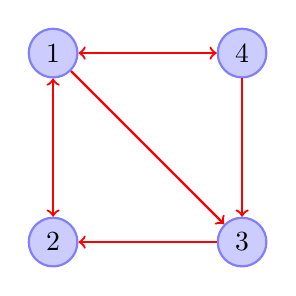
\begin{tikzpicture}[scale=1.2]
        \node(A) at (0,0) [place] {2};
        \node(B) at (2,0) [place] {3};
        \node(C) at (2,2) [place] {4};
        \node(D) at (0,2) [place] {1};            
        \draw[red,thick,<->] (A.north) -- (D.south);
        \draw[red,thick,->]  (C.south) -- (B.north);
        \draw[red,thick,->]  (D.south east) -- (B.north west);
        \draw[red,thick,<->] (D.east) -- (C.west);
        \draw[red,thick,<-]  (A.east) -- (B.west);
      \end{tikzpicture}
    \end{center}
  \end{figure}
  
  若令
  $$
  a_{ij} = \left\{
    \begin{array}{ll}
      1, & \mbox{从$i$市到$j$市有1条单向航线},\\[0.1in]
      0, & \mbox{从$i$市到$j$市没有单向航线},
    \end{array}
  \right.
  $$  
  则该航线图可用矩阵表示为
  \begin{figure}[htbp]
    \centering
    \begin{tikzpicture}[scale=0.5]
      \matrix (M) [matrix of math nodes]  { 
        \MA = \\
      };
      \matrix(MM) [right=.5in of M, matrix of math nodes,nodes in empty cells,
      column sep=4ex,row sep=.05ex,ampersand replacement=\&,left delimiter=(,right delimiter=)] {
        0 \& 1 \& 1 \& 1\\
        1 \& 0 \& 0 \& 0\\
        0 \& 1 \& 0 \& 0\\
        1 \& 0 \& 1 \& 0\\
      };
      \node[above=2pt  of MM-1-1, blue]  {城市1};
      \node[above=2pt  of MM-1-2, blue]  {城市2};
      \node[above=2pt  of MM-1-3, blue]  {城市3};
      \node[above=2pt  of MM-1-4, blue]  {城市4};
      \node[left =12pt  of MM-1-1, blue]  {城市1};
      \node[left =12pt  of MM-2-1, blue]  {城市2};
      \node[left =12pt  of MM-3-1, blue]  {城市3};
      \node[left =12pt  of MM-4-1, blue]  {城市4};
    \end{tikzpicture}
  \end{figure}
\end{li}


\begin{li}
  设变量$x_1, x_2, \cd, x_n$与变量$y_1,y_2,\cd,y_m$满足:
  \begin{equation}\label{lt}
    \left\{
      \begin{array}{c}
        y_1  = a_{11} x_1 + a_{12} x_2 + \cd + a_{1n} x_n, \\[0.2cm]
        y_2  = a_{21} x_1 + a_{22} x_2 + \cd + a_{2n} x_n, \\[0.2cm]
        \vd \\[0.2cm]
        y_m  = a_{m1} x_1 + a_{m2} x_2 + \cd + a_{mn} x_n
      \end{array}
    \right.
  \end{equation}
  它表示一个从变量$x_1, x_2, \cd, x_n$到变量$y_1,y_2,\cd,y_m$的\red{线性变换}, 其系数$a_{ij}$构成矩阵$A=(a_{ij})_{m\times n}$。
\end{li}
\begin{itemize}
\item  给定了线性变换(\ref{lt}),其\red{系数矩阵}也就确定。 
\item   反之,若给出一个矩阵作为线性变换的系数矩阵,则线性变换也就确定。 
\item   从这个意义上讲,线性变换与矩阵之间存在一一对应的关系。
\end{itemize}      

(1)、线性变换
$$
\left\{
  \begin{array}{c}
    y_1 = x_1, \\[0.2cm]
    y_2 = x_2, \\[0.2cm]
    \vd \\[0.2cm]
    y_n = x_n
  \end{array}
\right.
$$
称为\red{恒等变换}, 它对应$n$阶方阵
$$
\mathbf{I} = \left(
  \begin{array}{cccc}
    1    & 0    & \cd  & 0 \\
    0    & 1    & \cd  & 0 \\
    \vd  & \vd  &      & \vd \\
    0    & 0    & \cd  & 1
  \end{array}
\right). 
$$ 
该方阵称为$n$阶\red{单位矩阵},简称\red{单位阵}。其$(i,j)$元为
$$
\delta_{ij} = \left \{
  \begin{array}{ll}
    1, &i=j, \\
    0, &i\ne j.
  \end{array}
\right.  
$$

(2)、线性变换
$$
\left\{
  \begin{array}{c}
    y_1 = \lambda_1 x_1, \\[0.2cm]
    y_2 = \lambda_2 x_2, \\[0.2cm]
    \vd \\[0.2cm]
    y_n = \lambda_n x_n
  \end{array}
\right.
$$  
对应于$n$阶方阵
$$
\MA = \left(
  \begin{array}{cccc}
    \lambda_1& 0    & \cd  & 0 \\
    0    & \lambda_2    & \cd  & 0 \\
    \vd  & \vd  &      & \vd \\
    0    & 0    & \cd  & \lambda_n
  \end{array}
\right),
$$
这种方阵称为\red{对角矩阵},简称\red{对角阵},记作
$$
\MA = \mathrm{diag}(\lambda_1,\lambda_2,\cd,\lambda_n).
$$

(3)、  矩阵
$$
\left(
  \begin{array}{cc}
    1 & 0 \\
    0 & 0 
  \end{array}
\right)
$$ 
所对应的线性变换为
$$
\left\{
  \begin{array}{l}
    x_1 = x, \\[0.2cm]
    y_1 = 0
  \end{array}
\right.
$$
是一个投影变换。 
\begin{figure}[htbp]
  \centering
  \begin{tikzpicture}[scale=1.0]
    %% \draw[help lines] (0,0) grid (3,3);
    \draw[<->] (0,3) node[left] {$y$} -- (0,0) -- (3,0)node[below] {$x$};
    \node[label=-150:$O$]        (P0) at (0,0) {};
    \node[label=below:$P_1$] (P1) at (2,0) {};
    \node[label=above:$P$] (P) at (2,2.5) {};
    \draw[red, thick, ->] (P0.center) -- (P1.center);
    \draw[red, thick, ->] (P0.center) -- (P.center);
    \draw[red, thick, dashed] (P.center) -- (P1.center);
  \end{tikzpicture}
\end{figure}

(4)、    矩阵
$$
\left(
  \begin{array}{rr}
    \cos \varphi & -\sin \varphi \\
    \sin \varphi &  \cos \varphi 
  \end{array}
\right)
$$  
对应的线性变换
$$
\left \{
  \begin{array}{l}
    x_1 = x \cos \varphi - y \sin \varphi, \\[0.2cm]
    y_1 = x \sin \varphi + y \cos \varphi, \\[0.2cm]
  \end{array}
\right.
$$
设$x=r\cos \theta, y = r\sin \theta$,
则
$$
\begin{array}{l}
  x_1 = r(\cos\varphi \cos\theta - \sin\varphi \sin\theta) = r\cos(\theta+\varphi), \\[0.2cm]
  y_1 = r(\sin\varphi \cos\theta + \cos\varphi \sin\theta) = r\sin(\theta+\varphi), 
\end{array}
$$

\begin{figure}[htbp]
  \centering
  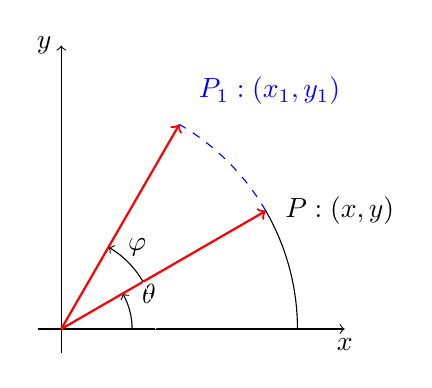
\begin{tikzpicture}[scale=3]
    % \draw[step=.5cm,gray,very thin] (-0.1,-0.1) grid (1.4,1.4);
    \draw[->] (-.1,0) -- (1.2,0)  node[below] {$x$};
    \draw[->] (0,-0.1) -- (0,1.2) node[left] {$y$};
    \draw[]   (1,0) arc (0:30:1) node(P)[label=right:$P:{(x,y)}$]{};
    \draw[->] (3mm,0mm) -- (3mm,0mm) arc (0:30:3mm) node(A)[label=right:$\theta$]{};
    \draw[red, thick, ->] (0,0) --  (P.center);
    
    \draw[white] (4mm,0mm) -- (4mm,0mm) arc (0:30:4mm) node(A){};
    \draw[->] (A.center) arc (30:60:4mm) node[label=right:$\varphi$]{};
    
    \draw[blue, dashed]  (P) arc (30:60:1) node(P1)[label=above right:$P_1:{(x_1,y_1)}$]{};
    
    \draw[red, thick, ->] (0,0) -- (P1.center);    
  \end{tikzpicture}
\end{figure}
这表明经过上述变换,将向量$OP$逆时针旋转$\varphi$角得到向量$OP_1$.


\begin{li}
  求解线性方程组
  $$
  \left\{
    \begin{array}{rcrcrcrcrr}
      2x_1 & - & 2x_2 &   &      & + &  6x_4 & = &-2 \\[0.1cm]
      2x_1 & - &  x_2 & + & 2x_3 & + &  4x_4 & = &-2 \\[0.1cm]
      3x_1 & - &  x_2 & + & 4x_3 & + &  4x_4 & = &-3 \\[0.1cm]
      5x_1 & - & 3x_2 & + &  x_3 & + & 20x_4 & = &-2 
    \end{array}
  \right.
  $$
\end{li}
\begin{jie}
  $$
  \left\{
    \begin{array}{rcrcrcrcrr}
      x_1 & - &  x_2 &   &      & + &  3x_4 & = &-1 \\[0.1cm]
          &  &  x_2 & + & 2x_3 & - &  2x_4 & = &0 \\[0.1cm]
          &  & 2x_2 & + & 4x_3 & - &  5x_4 & = &0 \\[0.1cm]
          &  & 2x_2 & + &  x_3 & + &  5x_4 & = &3 
    \end{array}
  \right.
  $$    
  $$
  \left\{
    \begin{array}{rcrcrcrcrr}
      x_1 & - &  x_2 &   &      & + &  3x_4 & = &-1 \\[0.1cm]
          &  &  x_2 & + & 2x_3 & - &  2x_4 & = &0 \\[0.1cm]
          &  &  &  &  & - &  x_4 & = &0 \\[0.1cm]
          &  &  & - &  3x_3 & + &  9x_4 & = &3 
    \end{array}
  \right.
  $$    
  $$
  \left\{
    \begin{array}{rcrcrcrcrr}
      x_1 & - &  x_2 &   &      & + &  3x_4 & = &-1 \\[0.1cm]
          &  &  x_2 & + & 2x_3 & - &  2x_4 & = &0 \\[0.1cm]
          &  &  & - &  3x_3 & + &  9x_4 & = &3 \\[0.1cm]
          &  &  &  &  & - &  x_4 & = &0 
    \end{array}
  \right.
  $$    
  $$
  \left\{
    \begin{array}{rcrcrcrcrr}
      x_1 & - &  x_2 &   &      & + &  3x_4 & = &-1 \\[0.1cm]
          &  &  x_2 & + & 2x_3 & - &  2x_4 & = &0 \\[0.1cm]
          &  &  &  &  x_3 & - &  3x_4 & = &-1 \\[0.1cm]
          &  &  &  &  &  &  x_4 & = &0 
    \end{array}
  \right.
  $$    
  如此形状的方程组称为\red{阶梯形线性方程组}.
  该方程组可写成矩阵形式
  \begin{figure}[htbp]
    \centering
    \begin{tikzpicture}
      \matrix(M) [matrix of math nodes,nodes in empty cells,,ampersand replacement=\&,left delimiter=(,right delimiter=)]{
        A \& \& b \\
      };
      \draw[dashed] (M-1-2.north) -- (M-1-2.south);
      \matrix(M1) [right=.1in of M,matrix of math nodes]{
        = \\
      };
      \matrix(MM) [right=.1in of M1,matrix of math nodes,nodes in empty cells,
      column sep=1ex,row sep=.5ex,ampersand replacement=\&,left delimiter=(,right delimiter=)] {
        2 \& -2 \& 0 \&  6 \& \& -2\\
        2 \& -1 \& 2 \&  4 \& \& -2\\
        3 \& -1 \& 4 \&  4 \& \& -3\\
        5 \& -3 \& 1 \& 20 \& \& -2\\
      };
      \draw[dashed] (MM-1-5.north) -- (MM-4-5);
    \end{tikzpicture}
    \caption{增广矩阵}
  \end{figure}
  求解过程可表示为
  \begin{figure}[htbp]
    \centering
    \begin{tikzpicture}          
      \matrix(A) [matrix of math nodes,nodes in empty cells,
      column sep=1ex,row sep=.1ex,ampersand replacement=\&,left delimiter=(,right delimiter=)] {
        A \& \& b \\
      };
      \draw[dashed] (A-1-2.north) -- (A-1-2.south);
      % \end{tikzpicture}
      
      % \begin{tikzpicture}
      \matrix (EQ1) [right=.1in of A,matrix of math nodes]  { 
        \xlongequal[]{\ds r_1 \div 2} \\
      };
      
      \matrix(A1) [right=.1in of EQ1,matrix of math nodes,nodes in empty cells, column sep=1ex,row sep=.1ex,ampersand replacement=\&,left delimiter=(,right delimiter=)] {
        1 \& -1 \& 0 \&  3 \& \& -1\\
        2 \& -1 \& 2 \&  4 \& \& -2\\
        3 \& -1 \& 4 \&  4 \& \& -3\\
        5 \& -3 \& 1 \& 20 \& \& -2\\
      };
      \draw[dashed] (A1-1-5.north) -- (A1-4-5);
      % \end{tikzpicture}

      
      % \begin{tikzpicture}
      
      \matrix(A2) [below=.1in of A1,matrix of math nodes,nodes in empty cells,
      column sep=1ex,row sep=.1ex,ampersand replacement=\&,left delimiter=(,right delimiter=)] {
        1 \& -1 \& 0 \&  3 \& \& -1\\
        0 \&  1 \& 2 \& -2 \& \&  0\\
        0 \&  0 \& 0 \& -1 \& \&  0\\
        0 \&  0 \&-3 \&  9 \& \&  3\\
      };
      \draw[dashed] (A2-1-5.north) -- (A2-4-5);
      \matrix (EQ2) [left=.1in of A2,matrix of math nodes]  { 
        \xlongequal[
        \ds r_3+(-3)\times r_1 \atop 
        \ds r_4+(-5)\times r_1]{\ds r_2+(-2)\times r_1} \\
      };

      % \end{tikzpicture}

      
      % \begin{tikzpicture}
      \matrix(A3) [below=.1in of A2,matrix of math nodes,nodes in empty cells,
      column sep=1ex,row sep=.1ex,ampersand replacement=\&,left delimiter=(,right delimiter=)] {
        1 \& -1 \& 0 \&  3 \& \& -1\\
        0 \&  1 \& 2 \& -2 \& \&  0\\
        0 \&  0 \&-3 \&  9 \& \&  3\\
        0 \&  0 \& 0 \& -1 \& \&  0\\
      };
      \draw[dashed] (A3-1-5.north) -- (A3-4-5);

      \matrix (EQ3) [left=.1in of A3,matrix of math nodes]  { 
        \xlongequal[]{\ds r_3 \leftrightarrow r_4} \\
      };

      
      \matrix(A4) [below=.1in of A3,matrix of math nodes,nodes in empty cells,
      column sep=1ex,row sep=.1ex,ampersand replacement=\&,left delimiter=(,right delimiter=)] {
        1 \& -1 \& 0 \&  3 \& \& -1\\
        0 \&  1 \& 2 \& -2 \& \&  0\\
        0 \&  0 \& 1 \& -3 \& \& -1\\
        0 \&  0 \& 0 \&  1 \& \&  0\\
      };
      \draw[dashed] (A4-1-5.north) -- (A4-4-5);

      \matrix (EQ4) [left=.1in of A4,matrix of math nodes]  { 
        \xlongequal[]{\ds r_3 \div (-3)} \\
      };
    \end{tikzpicture}
  \end{figure}
\end{jie}

\begin{li}
  求解线性方程组
  $$
  \left\{
    \begin{array}{rcrcrcrcrcrr}
      x_1 & - &  x_2 & - &  x_3 &   &       & + & 3x_5 & = &-1 \\[0.1cm]
      2x_1 & - & 2x_2 & - &  x_3 & + &  2x_4 & + & 4x_5 & = &-2 \\[0.1cm]
      3x_1 & - & 3x_2 & - &  x_3 & + &  4x_4 & + & 5x_5 & = &-3 \\[0.1cm]
      x_1 & - &  x_2 & + &  x_3 & + &   x_4 & + & 8x_5 & = & 2 
    \end{array}
  \right.
  $$
\end{li}
\newpage
\begin{jie}
  
  其增广矩阵为
  \begin{figure}[htbp]
    \centering
    \begin{tikzpicture}
      \matrix(Ab) [matrix of math nodes,nodes in empty cells,,ampersand replacement=\&,left delimiter=(,right delimiter=)]{
        A \& \& b \\
      };
      \draw[dashed] (Ab-1-2.north) -- (Ab-1-2.south);
      \matrix (EQ) [right=.1in of Ab,matrix of math nodes]  { 
        =\\
      };
      \matrix(A) [right=.1in of EQ,matrix of math nodes,nodes in empty cells,   column sep=1ex,row sep=.1ex,ampersand replacement=\&,left delimiter=(,right delimiter=)] {
        1 \& -1 \& -1 \&  0 \& 3 \& \& -1\\
        2 \& -2 \& -1 \&  2 \& 4 \& \& -2\\
        3 \& -3 \& -1 \&  4 \& 5 \& \& -3\\
        1 \& -1 \&  1 \&  1 \& 8 \& \&  2\\
      };
      \draw[dashed] (A-1-6.north) -- (A-4-6);
    \end{tikzpicture}      
  \end{figure}
  
  求解过程可表示为:
  \begin{figure}[htbp]
    \centering
    \begin{tikzpicture}
      \matrix(A) [matrix of math nodes,nodes in empty cells,,ampersand replacement=\&,left delimiter=(,right delimiter=)]{
        A \& \& b \\
      };
      \draw[densely dashed] (A-1-2.north) -- (A-1-2.south);
      \matrix (EQ1) [right=.1in of A,matrix of math nodes]  { 
        \xlongequal[\ds r_3+(-3)\times \ds r_1 \atop \ds r_4+(-1)\times r_1]{\ds r_2+(-2)\times r_1}\\
      };        
      \matrix(A1) [right=.1in of EQ1,matrix of math nodes,nodes in empty cells,
      column sep=1ex,row sep=.1ex,ampersand replacement=\&,left delimiter=(,right delimiter=)] {
        1 \& -1 \& -1 \&  0 \& 3 \& \& -1\\
        0 \&  0 \&  1 \&  2 \&-2 \& \&  0\\
        0 \&  0 \&  2 \&  4 \&-4 \& \&  0\\
        0 \&  0 \&  2 \&  1 \& 5 \& \&  3\\
      };
      \draw[dashed] (A1-1-6.north) -- (A1-4-6);

      \matrix(A2) [below=.1in of A1,matrix of math nodes,nodes in empty cells,
      column sep=1ex,row sep=.1ex,ampersand replacement=\&,left delimiter=(,right delimiter=)] {
        1 \& -1 \& -1 \&  0 \& 3 \& \& -1\\
        0 \&  0 \&  1 \&  2 \&-2 \& \&  0\\
        0 \&  0 \&  0 \&  0 \& 0 \& \&  0\\
        0 \&  0 \&  0 \& -3 \& 9 \& \&  3\\
      };
      \draw[dashed] (A2-1-6.north) -- (A2-4-6);
      \matrix (EQ2) [left=.1in of A2,matrix of math nodes]  { 
        \xlongequal[\ds r_3+(-2)\times r_2]{\ds r_3+(-2)\times r_2}\\
      };

      \matrix(A3) [below=.1in of A2,matrix of math nodes,nodes in empty cells,
      column sep=1ex,row sep=.1ex,ampersand replacement=\&,left delimiter=(,right delimiter=)] {
        1 \& -1 \& -1 \&  0 \& 3 \& \& -1\\
        0 \&  0 \&  1 \&  2 \&-2 \& \&  0\\
        0 \&  0 \&  0 \&  1 \& -3 \& \& -1\\
        0 \&  0 \&  0 \&  0 \& 0 \& \&  0\\
      };
      \draw[dashed] (A3-1-6.north) -- (A3-4-6);
      \matrix (EQ3) [left=.1in of A3,matrix of math nodes]  { 
        \xlongequal[\ds r_3 \leftrightarrow r_4]{\ds r_4\div(-3)}\\
      };
    \end{tikzpicture}           
  \end{figure}
  
  该矩阵称为\red{行简化阶梯矩阵},对应的线性方程组为
  $$
  \left\{
    \begin{array}{rcrcrcrcrcrr}
      x_1 & - &  x_2 &   &      &   &       & + & 7x_5 & = & 1 \\[0.1cm]
          &   &     &   &  x_3 &   &     & + & 4x_5 & = & 2 \\[0.1cm]
          &   &   &   &    &   &   x_4 & - & 3x_5 & = &-1
    \end{array}
  \right.
  $$
  \begin{zhu}
    该方程组有$5$个未知量,其中$x_1,x_3,x_4$为\red{基本未知量},$x_2,x_5$为\red{自由未知量}。
  \end{zhu}

  任取$x_2=k_1, x_5=k_2$,可得线性方程组的全部解
  $$
  \left\{
    \begin{array}{ccl}
      x_1 &=& 1+k_1-7k_2, \\[0.1cm]      
      x_2 &=& k_1, \\[0.1cm]
      x_3 &=& 2-4k_2, \\[0.1cm]
      x_4 &=& -1+3k_2,\\[0.1cm]
      x_5 &=& k_2.
    \end{array}
  \right.
  $$

\end{jie}

\begin{li}
  解线性方程组
  $$
  \left\{
    \begin{array}{rcrcrcr}
      x_1 & + & x_2 & + &  x_3 & = & 1, \\[0.1cm]
      x_1 & + &2x_2 & - & 5x_3 & = & 2, \\[0.1cm]
      2x_1 & + &3x_2 & - & 4x_3 & = & 5.
    \end{array}
  \right.
  $$
\end{li}
\newpage
\begin{jie}
  
  \begin{figure}[htbp]
    \centering
    \begin{tikzpicture}        
      \matrix(Ab) [matrix of math nodes,nodes in empty cells,
      column sep=1ex,row sep=.5ex,ampersand replacement=\&,left delimiter=(,right delimiter=)] {
        1 \&  1 \&  1 \& \&  1\\
        1 \&  2 \& -5 \& \&  2\\
        2 \&  3 \& -4 \& \&  5\\
      };
      \draw[dashed] (Ab-1-4.north) -- (Ab-3-4);
      
      \matrix (EQ1) [right=.1in of Ab,matrix of math nodes]  { 
        \xlongequal[r_3+ (-2)\times r_1]{r_2+ (-1)\times r_1}\\
      };

      \matrix(Ab1) [right=.1in of EQ1,matrix of math nodes,nodes in empty cells, column sep=1ex,row sep=.5ex,ampersand replacement=\&,left delimiter=(,right delimiter=)] {
        1 \&  1 \&  1 \& \&  1\\
        0 \&  1 \& -6 \& \&  1\\
        0 \&  1 \& -6 \& \&  3\\
      };
      \draw[dashed] (Ab1-1-4.north) -- (Ab1-3-4);

      \matrix (EQ2) [right=.1in of Ab1,matrix of math nodes]  { 
        \xlongequal[]{r_3+ (-1)\times r_2}\\
      };
      \matrix(Ab2) [right=.1in of EQ2,matrix of math nodes,nodes in empty cells,column sep=1ex,row sep=.5ex,ampersand replacement=\&,left delimiter=(,right delimiter=)] {
        1 \&  1 \&  1 \& \&  1\\
        0 \&  1 \& -6 \& \&  1\\
        0 \&  0 \&  0 \& \&  2\\
      };
      \draw[dashed] (Ab2-1-4.north) -- (Ab2-3-4);        
    \end{tikzpicture}
  \end{figure}
  
  由第三行可以看出,该线性方程组无解。
\end{jie}

\begin{itemize}
\item 含有矛盾方程而无解的方程组称为\red{不相容方程组};
\item 有解的方程组称为\red{相容方程组};
\item \red{多余方程}。
\end{itemize}

对于一般的线性方程组
$$
\left\{
  \begin{array}{c}
    a_{11}x_1 + a_{12}x_2 + \cd + a_{1n}x_n = b_1\\[0.2cm]
    a_{21}x_1 + a_{22}x_2 + \cd + a_{2n}x_n = b_2\\[0.2cm]
    \vd\\[0.2cm]
    a_{m1}x_1 + a_{m2}x_2 + \cd + a_{mn}x_n = b_m
  \end{array}
\right.
$$

其增广矩阵为
\begin{figure}[htbp]
  \centering
  \begin{tikzpicture}
    \matrix(MM) [matrix of math nodes,nodes in empty cells,
    column sep=1ex,row sep=.5ex,ampersand replacement=\&,left delimiter=(,right delimiter=)] {
      a_{11} \&  a_{12} \&  \cd \& a_{1n} \& \&  b_1\\
      a_{21} \&  a_{22} \&  \cd \& a_{2n} \& \&  b_2\\
      \vd   \&  \vd   \&      \&  \vd  \& \& \vd \\
      a_{m1} \&  a_{m2} \&  \cd \& a_{mn} \& \&  b_m\\
    };
    \draw[dashed] (MM-1-5.north) -- (MM-4-5);        
  \end{tikzpicture}      
\end{figure}
对于以上增广矩阵,总是可以经过一系列的变换将其化成
\begin{figure}[htbp]
  \centering
  \begin{tikzpicture}
    \matrix(MM) [matrix of math nodes,nodes in empty cells,
    column sep=0.6ex,row sep=.5ex,ampersand replacement=\&,left delimiter=(,right delimiter=)] {
      a_{11} \&  a_{12} \&  \cd \& a_{1n} \& \&  b_1\\
      a_{21} \&  a_{22} \&  \cd \& a_{2n} \& \&  b_2\\
      \vd   \&  \vd   \&      \&  \vd  \& \& \vd \\
      a_{m1} \&  a_{m2} \&  \cd \& a_{mn} \& \&  b_m\\
    };
    \draw[dashed] (MM-1-5.north) -- (MM-4-5);
    
    \matrix (M2) [right=.05in of MM,matrix of math nodes]  { 
      \Rightarrow\\
    };
    
    \matrix(MM) [right=.05in of M2,matrix of math nodes,nodes in empty cells,
    column sep=0.6ex,row sep=.5ex,ampersand replacement=\&,left delimiter=(,right delimiter=)] {
      c_1 \&   0 \& \cd \&  0 \& c_{1,r+1} \& \cd \& c_{1n} \& \& d_1\\
      0   \& c_2 \& \cd \&  0 \& c_{2,r+1} \& \cd \& c_{2n} \& \& d_2\\
      \vd \& \vd \& \dd \&\vd \& \vd     \&     \& \vd   \& \& \vd\\
      0   \&  0  \& \cd \& c_{rr} \& c_{r,r+1} \& \cd \& c_{rn} \& \& d_r\\
      0   \&  0  \& \cd \& 0 \& 0 \& \cd \& 0 \&  \& d_{r+1}\\
      0   \&  0  \& \cd \& 0 \& 0 \& \cd \& 0 \&  \& 0\\          
      \vd \& \vd \& \dd \&\vd \& \vd     \&     \& \vd   \& \& \vd\\
      0   \&  0  \& \cd \& 0 \& 0 \& \cd \& 0 \&  \& 0\\
    };
    \draw[dashed] (MM-1-8.north) -- (MM-8-8);
    \filldraw[opacity=0.5,red!50] (MM-5-9) circle (0.3cm);
  \end{tikzpicture}      
\end{figure}
其中$c_{ii}=1~(i=1,2,\cd,r)$。对应线性方程组解的情况如下:   
\begin{itemize}
\item[1] 线性方程组有解$ \Leftrightarrow \red{d_{r+1}=0}$;\\[0.3cm]
\item[2] 在有解的情况下:
  \begin{itemize}
  \item 当$r=n$时,有唯一解$x_1=d_1,~x_2=d_2,~\cd,~x_n=d_n$;
  \item 当$r<n$时,有无穷多解
    $$
    \left\{
      \begin{array}{ccl}
        x_1 &=& d_1 - c_{1,r+1}k_1 - \cd - c_{1n}k_{n-r}, \\[0.1cm]
        x_2 &=& d_2 - c_{2,r+1}k_1 - \cd - c_{2n}k_{n-r}, \\[0.1cm]
        \vd & & \vd \\[0.1cm]
        x_r &=& d_r - c_{r,r+1}k_1 - \cd - c_{rn}k_{n-r}, \\[0.1cm]
        x_{r+1} &=& k_1, \\[0.1cm]
        \vd && \vd \\[0.1cm]
        x_{n} &=& k_{n-r}.
      \end{array}
    \right.
    $$
  \end{itemize}
\end{itemize}
